\section{Тестирование мультимодальности генеральной совокупности}

Наш второй пример гораздо более экзотичен. Это случай, когда не существует простых тестов, основанных на нормальном распределении, и нельзя использовать перестановочный тест, но можно эффективно использовать бутстреп. Данные представляют собой толщину в миллиметрах $485$ марок, напечатанных в $1872$ году. Выпуск марок того года считался <<филателистической смесью>>, то есть напечатанным на более чем одном типе бумаги. Исторический интерес представляет определение того, сколько различных типов бумаги использовалось.

Гистограмма данных показана в верхнем левом углу рисунка 16.2. Эта выборка является частью большой коллекции марок $1872$ года, и мы можем представить себе распределение измерений толщины для всей генеральной совокупности. Мы ставим статистический вопрос: сколько мод у этой генеральной совокупности? Мода определяется как локальный максимум или <<скачок>> плотности популяции. Количество мод указывает на количество различных типов бумаги, используемых при печати.

Из гистограммы на рисунке 16.2 видно, что популяция может иметь две или более мод. Однако это трудно сказать, потому что гистограмма не гладкая. Чтобы получить более гладкую оценку, мы можем использовать \textit{ядерную оценку плотности с использованием функции Гаусса}. При обозначении данных как $\xes{n}$, Гауссова плотность распределения определяется выражением
\begin{equation}\label{eq16.19}
    \hat{f}(t;\,h) = \frac{1}{nh}\sum\limits_{1}^{n}\phi\left(\frac{t-x_i}{h}\right),
\end{equation}
где $\phi(t)$ --- плотность стандартного нормального распределения $\frac{1}{\sqrt{2\pi}}\exp\left(-t^2/2\right)$. Параметр $h$ называется размером окна и определяет степень сглаживания, применяемого к данным. Чем больше значение $h$, тем более гладкая оценка плотности.

Мы можем думать о (\ref{eq16.19}) как о суммировании $n$ маленьких гауссовых кривых плотности с центрами в каждой точке $x_i$, каждая из которых имеет стандартное отклонение $h$; рисунок 16.3 иллюстрирует это.

На верхней правой части рисунка 16.2 показана итоговая оценка плотности с использованием $h = 0.003$; имеется две или три моды. Однако, изменяя $h$, мы можем получить большее или меньшее количество мод. Внизу слева и справа показаны оценки плотности, полученные с использованием $h = 0.008$ и $h = 0.001$ соответственно. На левом есть одна мода, а на правом как минимум семь! Очевидно, что вывод, который мы делаем из наших данных, сильно зависит от значения $h$, которое мы выбираем.

\newpage
\noindent
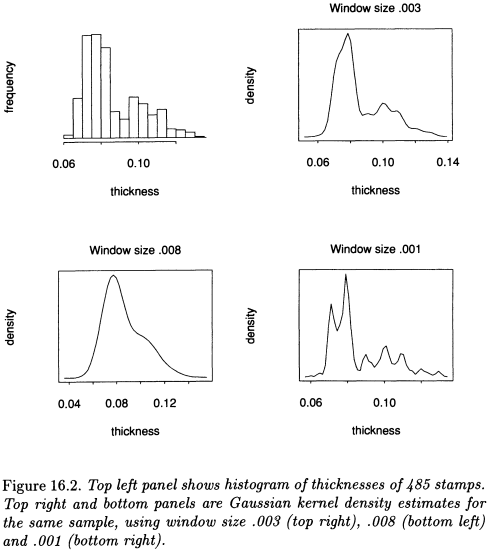
\includegraphics[width=\linewidth]{16/f16.2.png}

Если мы подойдем к проблеме с точки зрения проверки гипотез, есть естественный способ выбрать $h$. Нам понадобится следующий важный результат, который мы сформулируем без доказательства: с увеличением $h$ количество мод Гауссовой плотности не увеличивается. Это проиллюстрировано для данных о толщине марок на рисунке 16.4.

Теперь рассмотрим проверку
\begin{equation}\label{eq16.20}
    H_0: \text{число мод } = 1 
\end{equation}
против альтернативы количество мод $> 1$. Поскольку количество мод уменьшается с увеличением $h$, существует наименьшее значение $h$ такое, что $\hat{f}(t;\, h)$ имеет одну моду. Назовем его $\hat{h}_1$. Глядя на рисунок 16.4, можно сказать, что $\hat{h}_1 \approx 0.0068$.

Кажется разумным использовать $\hat{f}(t;\, h)$ в качестве оценки нулевого распределения для нашего тестирования $H_0$. В некотором смысле это оценка плотности, наиболее близкая к нашим данным, которая согласуется с $H_0$. Под <<ближайшая>> мы подразумеваем, что она использует наименьшее сглаживание (наименьшее значение $h$) среди всех оценок с одной модой.

\newpage
\noindent
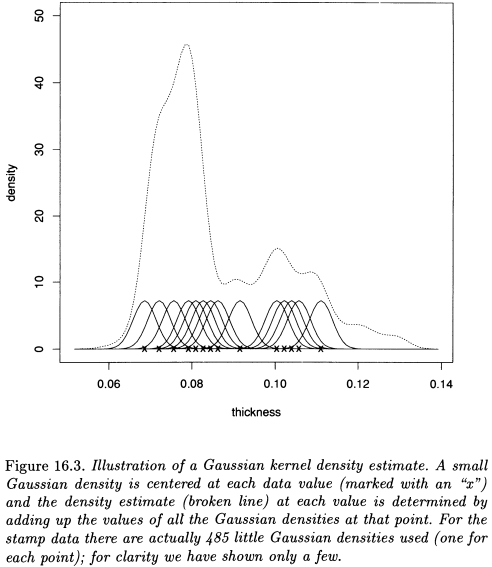
\includegraphics[width=\linewidth]{16/f16.3.png}

Есть одна небольшая поправка, которую мы вносим в $\hat{f}(\,\cdot\,;\, \hat{h}_1)$. Формула (\ref{eq16.19}) искусственно увеличивает дисперсию оценки, поэтому мы масштабируем ее так, чтобы дисперсия была равна дисперсии выборки. Обозначим измененную оценку через $\hat{g}(\,\cdot\,;\, \hat{h}_1)$.

Наконец, нам нужно выбрать тестовую статистику. Естественный выбор --- это $ \hat{h}_1$, наименьший размер окна, дающий оценку плотности с одной модой. Большое значение $ \hat{h}_1$ указывает на то, что необходимо выполнить большое сглаживание, чтобы получить оценку с одной модой, и, следовательно, является свидетельством против $H_0$.

Собирая все это вместе, бутстреп проверка гипотезы $H_0: \text{число мод } = 1$ основана на достижении уровня значимости
\begin{equation}\label{eq16.21}
    \text{ASL}_{\text{boot}} = \text{Prob}_{\hat{g}(\,\cdot\,;\, \hat{h}_1)}\left\{\hat{h}^{*}_1 > \hat{h}_1\right\}.
\end{equation}

Здесь $\hat{h}_1$ зафиксировано на наблюдаемом значении $0.0068$; бутстреп выборка $\xest{n}$ берется из $\hat{g}(\,\cdot\,;\, \hat{h}_1)$, а $\hat{h}^{*}_1$ --- наименьшее значение $h$, дающее оценку плотности с одной модой по бутстреп выборке $\xest{n}$.

\newpage
\noindent
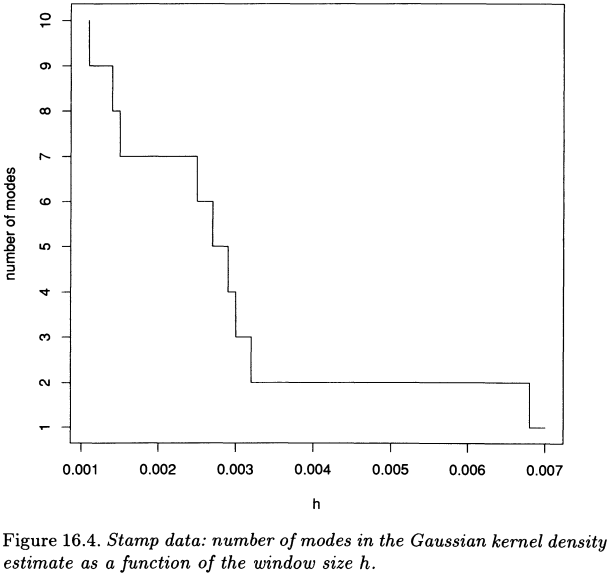
\includegraphics[width=\linewidth]{16/f16.4.png}

Чтобы аппроксимировать $\text{ASL}_{\text{boot}}$, нам нужно получить бутстреп выборки из масштабированной оценки плотности $\hat{g}(\,\cdot\,;\, \hat{h}_1)$. То есть, вместо того, чтобы производить выборку с возвращением, мы получаем выборку с помощью гладкой оценки плотности генеральной совокупности. Это называется гладким бутстрепом. Из-за удобной формы ядерной оценки плотности легко получить выборку из $\hat{g}(\,\cdot\,;\, \hat{h}_1)$. Выберем $y^{*}_1, y^{*}_2, \ldots, y^{*}_n$ с возвращением из $\xes{n}$ и положим
\begin{equation}\label{eq16.22}
    x^{*}_i = \bar{y}^{*} + \left(1+\hat{h}^2_1/\hat{\sigma}^2\right)^{-1/2}\left(y^{*}_i - \bar{y}^{*} + \hat{h}_1\epsilon_i\right);\quad i = \ies{n},
\end{equation}
где $\bar{y}^{*}$ --- среднее значение $y^{*}_1, y^{*}_2, \ldots, y^{*}_n$, $\hat{\sigma}^2$ --- оценка по методу подстановки дисперсии, а $\epsilon_i$ --- стандартные нормальные случайные величины. Множитель $$\left(1+\hat{h}^2_1/\hat{\sigma}^2\right)^{-1/2}$$ масштабирует оценку так, чтобы его дисперсия была приблизительно равна $\hat{\sigma}^2$. Краткое изложение шагов показано в алгоритме 16.3.

Мы выполнили этот процесс с $B = 500$. Из $500$ бутстреп выборок ни одна не имела $\hat{h}^{*}_1 > 0.0068$, поэтому $\text{ASL}_{\text{boot}} = 0$. Мы повторили процесс для $H_0: \text{число мод} = 2, 3, \ldots$, и таблица 16.1 показывает итоговые $p$-значения. Интерпретируя эти результаты последовательно, начиная с $\text{числа мод} = 1$, мы отвергаем гипотезу об одной моде, но не отвергаем гипотезу двух модах. На этом процесс рассуждений во многих случаях заканчивался. Если бы мы были готовы принять более экзотические гипотезы, то из таблицы 16.1 также можно было бы предположить, что в генеральной совокупности может быть семь мод.

\begin{center}
    \textit{Алгоритм 16.3}
\end{center}
\fbox{%
\parbox{\textwidth}{%
\begin{center}
    \underline{Вычисление статистики для бутстреп проверки гипотезы о мультимодальности}
\end{center}
\begin{enumerate}
        \item Получить $B$ выборок размера $n$ из $\hat{g}(\,\cdot\,;\, \hat{h}_1)$ используя (\ref{eq16.22}).
        \item Для каждой бутстреп выборки вычислить наименьшую ширину окна, которая дает оценку плотности с одной модой. Обозначим $B$ значений $\hat{h}^{*}_1$ через $\hat{h}^{*}_1(1), \ldots, \hat{h}^{*}_1(B)$.
        \item Аппроксимировать $\text{ASL}_{\text{boot}}$ с помощью
        \begin{equation}\label{16.23}
            \widehat{\text{ASL}}_{\text{boot}} = \#\left\{\hat{h}^{*}_1(b) \geq \hat{h}_1\right\}/B.
        \end{equation}
    \end{enumerate}}%
}\\

\noindent
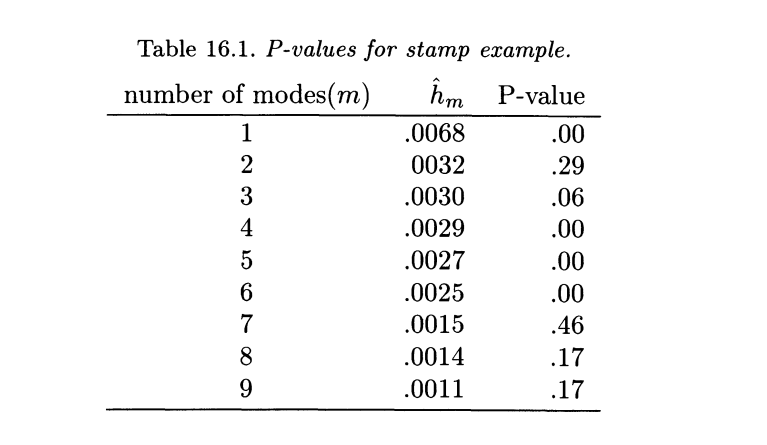
\includegraphics[width=\linewidth]{16/t16.1.png}









